\documentclass[String-lecture-21.tex]{subfiles}

\begin{document}\section{Type I superstring theory}\label{sec:TypeI}



So far we have considered oriented world-sheet Riemann surfaces.
However, it is quite natural to consider processes in Figure \ref{unoriented-WS}, which yields an unoriented world-sheet.
\begin{figure}[htb]
 \centerline{\includegraphics[width=9cm]{picture/unoriented-WS}}
\caption{Unoriented processes. The left is open string one, and the right is closed string one.}
\label{unoriented-WS}
\end{figure}
Therefore, we will consider the so-called \textbf{unoriented string},
which leads to Type I superstring theory. As we will see below, an unoriented string theory needs to incorporate open strings.



Open strings can end on D-branes in Type II theories. However, without D-branes, Type II theories cannot incorporate open strings
due to supersymmetry as follows. In fact, $D=10$
$\cN=2$ supersymmetry requires $\textbf{8}_v$ to have two superpartners
as like for a graviton to have two gravitinos in Table \ref{tab:masslessII}.
On the other hand, after the GSO projection, open strings can have one of the following massless states:
\begin{align*}
 &P_\mathrm{GSO}: \quad \mathrm{NS}, \ \mathrm{R+} = \textbf{8}_v +\textbf{8}_s \ ,  \\
 &\wt P_\mathrm{GSO}: \quad \mathrm{NS}, \ \mathrm{R-} = \textbf{8}_v +\textbf{8}_c \ ,
\end{align*}
where $\textbf{8}_v$ represents a gauge field and $\textbf{8}_{s,c}$ are gauginos.
Hence, the gauge field has only one superpartner so that it cannot exist in Type II theories without D-branes.


In fact, the existence of (parallel) D-branes breaks a half of supersymmetries so that open strings can end on D-branes. To consider unoriented string theory, we will introduce an \textbf{orientifold plane} or \textbf{O-plane} that breaks a half of supersymmetry. With an O-plane, it is natural to consider unoriented open string theory.
Although the argument below mainly focuses on the bosonic string for simplicity, it is straightforward to apply for superstrings.



\subsection{Orientifold}\label{sec:orientifold}

As in Figure \ref{unoriented-WS}, an orientation flip exchanges
left- and right-movers for closed strings and a reversal of the spatial direction for open strings.


Let us first take a look at an orientation flip operator $\Omega$ on a bosonic closed string. It exchanges the left and right-moving modes which ends up with a reversal of  the spatial direction up to the overall sign:
\begin{align}\label{O-closed}
 \Omega :
 \begin{cases}
  X(t,\sigma) &\leftrightarrow \quad X(t,-\sigma) \\
  b(t,\sigma) &\leftrightarrow \quad \ol b(t,-\sigma)  \\
  c(t,\sigma) &\leftrightarrow \quad -\ol c(t,-\sigma)  \\
 \end{cases} \ , \qquad\qquad  \Omega :
  \begin{cases}
   \alpha^\mu_n &\leftrightarrow \quad \ol \alpha^\mu_n \\
   b_n &\leftrightarrow \quad \ol b_n  \\
   c_n &\leftrightarrow \quad \ol c_n  \\
  \end{cases} \ ,
\end{align}
where $t$ is the Euclidean world-sheet time, not $\tau$. Thus, the projection by the orientation flip, called an orientifold,
 keeps only $\Omega$ invariant states such as the tachyon vacuum, gravitons and dilaton, but it projects out the $B$-field. Since a closed string is electrically coupled to the $B$-field, this implies that an unoriented closed string is not stable and it should decay.

% With the remaining states, we can consider an amplitude including an unorientable world-sheet, such as a Klein bottle.

Now, let us introduce a space-filling D$25$-brane and consider an open string with the Neumann boundary condition. As in \eqref{open-variation}, the Neumann boundary condition identifies the left and right-moving modes. Then, the orientation flip operator acts as
\begin{align}\label{O-open}
 \Omega :
 \begin{cases}
  X(t,\sigma) &\leftrightarrow \quad X(t,\pi-\sigma) \\
  b(t,\sigma) &\leftrightarrow \quad \ol b(t,\pi-\sigma)  \\
  c(t,\sigma) &\leftrightarrow \quad -\ol c(t,\pi-\sigma)  \\
 \end{cases} \ ,\qquad\qquad
 \Omega :
 \begin{cases}
  \alpha^\mu_n &\leftrightarrow \quad (-1)^n \alpha^\mu_n \\
  b_n &\leftrightarrow \quad (-1)^n b_n  \\
  c_n &\leftrightarrow \quad (-1)^n c_n  \\
 \end{cases} \ ,
\end{align}
Now recall that we can incorporate Chan-Paton degrees of freedom \eqref{CP-factors} for open string states. The orientation flip $\Omega$ exchanges the Chan-Paton indices $i\leftrightarrow j$. Hence,
writing an open string state as in \eqref{CP-factor2}
\begin{align*}
 |N,k;T\rangle \equiv |N,k;ij\rangle T_{ij} \ ,
\end{align*}
$\Omega$ acts on the state as
\begin{align*}
 \Omega |N,k;T\rangle = (-1)^N|N,k;T^t\rangle \ .
\end{align*}
Therefore, it imposes the condition
\bea
 T^t = T & \quad \textrm{for } N \textrm{ even }\cr
 T^t =- T & \quad \textrm{for } N \textrm{ odd }~.
\eea
In particular, a gauge boson arises at level one \eqref{open-massless} so that we need to impose the anti-symmetric condition $ T^t =- T$ on the Chan-Paton factor. Consequently, it gives rise to a $\SO(n)$ gauge field.


In general, when orientation is flipped, we can also transform the Chan-Paton
index by a matrix $P$ at the same time.
\[\Omega|N ; k ; i j\rangle=(-1)^NP_{jj^{\prime}}\left|N ; k ; j^{\prime}i^{\prime} \right\rangle P_{i^{\prime}i}^{-1}\]
The projection operator is subject to $\Omega^2=1$, which gives the constraint
$$\Omega^{2}|N ; k ; i j\rangle=[(P^{T})^{-1} P]_{i i^{\prime}}\left|N ; k ; i^{\prime} j^{\prime}\right\rangle(P^{-1} P^{T})_{j^{\prime} j}~,\quad\Rightarrow \quad P^tP^{-1}=\pm1$$
Furthermore, there is a $\U(n)$ gauge equivalence relation $T \sim \wt T = UT U^{-1}$ $(U\in \U(n))$, which amounts to  $\wt P \sim U P U^t$,
Taking the gauge equivalence into account, $P^tP^{-1}=1$ leads to $P=1$, in which the gauge Lie algebra becomes $\SO(n)$ as above. On the other hand,
for $P^tP^{-1}=-1$, the rank needs to be even $n=2k$, and we can take a basis such that
\[P = i
       \begin{pmatrix}
        0 & -\textbf{1}_{k\times k}  \\
        \textbf{1}_{k\times k} & 0
       \end{pmatrix}\]
In this situation, the gauge Lie algebra becomes $\Sp(k)$ so that $T^t=-PTP$. We denote the orientifold flip projections that give rise to an SO and Sp gauge group by an O${}^-$- and O${}^+$-plane, respectively.



\subsubsection*{Unoriented superstring spectrum}

Now, let us consider the orientation flip operation $\Omega$ in superstring theories.
Since $\Omega$ exchanges the left- and right-moving modes, both must have the same spectra. Hence, it can only act on Type IIB theory but not on Type IIA theory. (See \eqref{IIA-IIB}.) The orientation flip projection of Type IIB theory is called \textbf{Type I superstring theory}.
In Table \ref{tab:masslessII}, the flip projects out the $B$-field $[2]$ in the NS-NS sector,
as well as a half of the NS-R R-NS sector $\textbf{8}_c + \textbf{56}_s$ (only the diagonal part survives).
Supersymmetry requires that the number of bosons and fermions are the same,
which implies that $[0]$ and $[4]_+$ are eliminated
and only the second rank anti-symmetric field $[2]$ survives in the R-R sector. This implies that $\Omega$ projects out D$(-1)$-, D$3$-, D$7$-branes. Then,  D$1$- and D$5$-branes are electrically and magnetically coupled to the R-R two-form $C_{(2)}$, respectively.
The remaining states are
\begin{align*}
 [0] \oplus [2] \oplus(2) \oplus\textbf{8}_c \oplus\textbf{56} =& \textbf{1} \oplus\textbf{28} \oplus\textbf{35} \oplus\textbf{8}_c \oplus\textbf{56}_s  \cr
 & \Phi \quad C_{\mu\nu} \ \ G_{\mu\nu}  \ \  \lambda^-  \ \ \ \psi_\mu^+ \
\end{align*}
Furthermore, to incorporate open-strings $\textbf{8}_v +\textbf{8}_s$, Type I theory incorporates space-filling non-dynamical D9-Branes. The orientation flip operation $\Omega$ can be understood as the effect of an O9-plane.

In conclusion, Type I is an unoriented, open plus closed superstring theory in which the massless spectrum is
\begin{align*}
  [0] \oplus [2] \oplus (2) \oplus\textbf{8}_c \oplus\textbf{56} \oplus(\textbf{8}_v \oplus\textbf{8}_s)_{\SO(n) \textrm{ or } \Sp(n)} \ .
\end{align*}
However, there is one important quantum effect we need to take into account. An O9-plane has R-R charge that has to cancel with the charge of D9-branes. From the world-sheet perspective, this corresponds to the \textbf{tadpole cancellation}.
In what follows, we will investigate the tadpole cancellation in bosonic string theory, and will see that the gauge group needs to be $\SO(2^{13})$. A similar analysis tells us that the gauge group must be  $\SO(32)$ in Type I superstring theory.




\subsection{Amplitude of Type I theory}


As above, unoriented open strings give rise to either $\SO(n)$ or $\Sp(n)$ massless gauge fields.
However, unless the tadpole cancellation is satisfied, the theory is still anomalous. We will see it in bosonic string theory.


\subsubsection*{Cylinder}
First, let us evaluate an ``oriented'' open string one-loop amplitude where a world-sheet is a cylinder (or annulus) as in the left of Figure \ref{oriented-unoriented}. We consider that there are $n$ D$25$-branes (or D$9$-branes for superstring) so that all of the boundary conditions are of Neumann type. The evaluation is parallel to \S\ref{sec:amplitude}.
\begin{figure}[htb]
\centerline{\includegraphics[width=\textwidth]{picture/oriented-unoriented}}
\caption{Cylinder, Klein bottle and M\"obius strip.}
\label{oriented-unoriented}
\end{figure}
It is clear from Figure \ref{oriented-unoriented} that we notice the following facts:
\vspace{-4pt}
\begin{itemize}
% \setlength{\parskip}{0cm}
 \setlength{\itemsep}{0pt}
 \item The range is $0 \le \Re~w \le \pi$, the period is $w \sim w +2\pi il$.
 \item There is a real modulus $l$ so that the amplitude needs one $b$ zero mode insertion.
 \item There is a translational isometry, a shift of $\Im~w$ so that  the amplitude needs one $c$ zero mode insertion.
\end{itemize}
Consequently, the cylinder partition function is written as
\begin{align*}
 A_{0,C} = \int \frac{dl}{2l} \langle b_0 c_0 \rangle_\mathrm{gh} \langle 1 \rangle_\mathrm{mat} \ ,
\end{align*}
where the ghost zero modes in open strings are read off
\begin{align*}
 &b_0 = \frac{1}{2\pi} \int_0^{\pi} \left[ dw\ b(w) +d\ol w\ \ol b(\ol w)\right] \ , \\
 &c_0 = \frac{i}{2\pi} \int_0^{\pi} \left[ dw\ c(w) -d\ol w\ \ol c(\ol w)\right] \ .
\end{align*}

Using operator formalism, we can derive each contribution as
\begin{align*}
 \langle 1 \rangle_\mathrm{mat} &= n^2\ \Tr \left[ q^{L_0^X -\frac{c}{24}} \right]= n^2 \cdot \frac{iV_{26}}{(2\pi)^{26}} (2l\alpha')^{-13} \cdot \eta(il)^{-26} \ ,  \\
 \langle b_0 c_0 \rangle_\mathrm{gh} &= \Tr \left[ (-1)^F b_0 c_0 q^{L_0^g-\frac{c}{24}} \right] = \eta(il)^2\ ,
\end{align*}
where $q=e^{-2\pi l}$ and the Virasoro generators are in \eqref{open-Virasoro} for open strings. Note that $n^2$ comes from the trace over the Chan-Paton degrees of freedom.
Therefore, the cylinder partition function  is
\begin{align}\label{cylinder}
 A_{0,C} = n^2 \cdot \frac{iV_{26}}{(2\pi \ell_s)^{26}}\int_0^\infty \frac{dl}{2l} \frac{1}{(2l)^{13} \eta(il)^{24}} \ ,
\end{align}
where $\ell_s = \sqrt{\alpha'}$ is the string length.

\begin{figure}[htb]
 \centerline{\includegraphics[width=13cm]{picture/openClosedAmp}}
 \caption{Pictorial description of the equivalence between open string one-loop and closed string propagation.}
 \label{fig:openClosedAmp}
\end{figure}


Let us look into its physical implication. When $l\to 0$, the cylinder becomes a thin tube, and it can be regarded as a propagation of a closed string as in Figure \ref{fig:openClosedAmp}. This is called the \textbf{open-closed duality}.
       This is justified by rewriting the amplitude. Using the modular property \eqref{S-T} of the Dedekind $\eta$-function, we can rewrite it in terms of $l=s^{-1}$ as
\be\label{cylinder2}
  A_{0,C} = \frac{n^2}{2^{13}} \cdot \frac{iV_{26}}{(2\pi \ell_s)^{26}} \int_0^\infty \frac{ds}2\ \eta(is)^{-24} \ ,
\ee
where
\[\eta(is)^{-24} = q^{-1} +24 +\cdots \equiv \sum_{N=0}^\infty \mathcal N_N q^{N-1} \quad (q = e^{-2\pi s}) \ .\]
In \eqref{cylinder}, there is an UV divergence from $l \to 0$, as opposed to the closed string case.
The UV divergence $l\to 0$ in an open string is replaced by the IR divergence $s \to \infty$ of a closed string propagation, which can be understood as particle propagations (sum of lines) as follows (see also Figure \ref{masslessProp}).
 \begin{align*}
  \int_0^\infty ds \sum_{N=0}^\infty \mathcal N_N e^{-2\pi s(N-1)}
  \sim  \sum_{i} \int_0^\infty ds\ e^{-s(k^2+m^2_i)} = \left. \sum_i \frac{1}{k^2+m^2_i} \right|_{k=0} \ .
 \end{align*}
       We can see that the IR divergence is from massless particle propagation (graviton etc.),
       which is absorbed or emitted from D$25$-branes. This point will be revisited at the end of \S\ref{sec:DBI}.
 In conclusion, the divergence is due to the existence of the D$25$-branes,
       which have definite tension (this is why they emit graviton/dilaton).
To cure this divergence, we will consider unoriented string amplitudes when world-sheets are Klein bottle and M\"obius strip as in  Figure \ref{oriented-unoriented}. The reason will become clear later.

\begin{figure}[htb]
 \centerline{\includegraphics[width=5cm]{picture/masslessProp}}
 \caption{Intermediate propagation is replaced by particles (lines).}
 \label{masslessProp}
\end{figure}


\subsubsection*{Klein bottle amplitude}
\begin{figure}[htb]
\centerline{\includegraphics[width=8cm]{picture/crosscap}}
\caption{$\bR P^2$ is obtained by identifying the antipodal points on $S^2$. This is equivalent to the southern hemisphere and the equators}
\label{crosscap}
\end{figure}
Next, let us evaluate an unoriented closed string one-loop amplitude when a world-sheet is a Klein bottle.
Since the Klein bottle can be realized by identifying the top and the bottom string by the orientation flip operator as in Figure \ref{KleinBottle},
the amplitude can be written as
\begin{align*}
 A_{0,K} = \int \frac{dl}{2l}
 \Tr \Bigl[ \Omega (-1)^F \frac{1}{2}(b_0+\ol b_0) \frac{1}{2}(c_0+\ol c_0) q^{L_0 +\ol L_0 -\frac{c}{12}} \Bigr] \qquad (q=e^{-2\pi l}) \ .
\end{align*}
Using \eqref{O-closed}, we can rewrite it as
\begin{align*}
 A_{0,K} = \frac{1}{2} \int \frac{dl}{2l}
 \Tr \left[ (-1)^F b_0 c_0 q^{2L_0^{\textrm{tot}}  -\frac{c^{\textrm{tot}}}{12}} \right] \ ,
\end{align*}
where $L_0$ and $c$ are the Virasoro generators and the central charge for closed strings.
Thus, the result is
\begin{align}\label{klein}
 A_{0,K} &= \frac{iV_{26}}{(2\pi \ell_s)^{26}} \int \frac{dl}{2l} \frac{1}{l^{13} \eta(2il)^{24}} = 2^{13} \frac{iV_{26}}{(2\pi \ell_s)^{26}} \int \frac{ds}{2} \eta(is)^{-24} \ .
\end{align}

\begin{figure}[htb]

\centerline{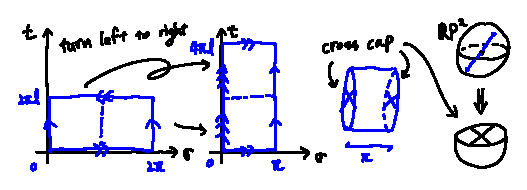
\includegraphics[width=13cm]{picture/KleinBottle}}
\caption{Klein bottle. It can be described by a cylinder with cross cap boundary on both ends.}
\label{KleinBottle}
\end{figure}

\subsubsection*{M\"obius strip amplitude}
\begin{figure}[htb]
\centerline{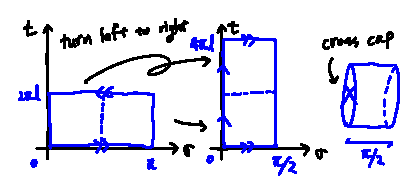
\includegraphics[width=13cm]{picture/MobiusStrip}}
\caption{M\"obius strip.}
\label{MobiusStrip}
\end{figure}

Finally, let us evaluate an unoriented open string one-loop amplitude when a world-sheet is a M\"obius strip. (See Figure \ref{MobiusStrip}.)
It has
\vspace{-4pt}
\begin{itemize}
% \setlength{\parskip}{0cm}
 \setlength{\itemsep}{0pt}
 \item The range is $0 \le \sigma \le \pi$, the period is $2\pi l$, coming together with the orientation flip:
       $(t,\sigma) \sim (t+2\pi l,\pi -\sigma)$.
 \item There is a real modulus $l$; the amplitude needs one $b$ zero mode insertion.
 \item There is a real isometry, which is the time translation; the amplitude needs one $c$ zero mode insertion.
\end{itemize}

Thus, the M\"obius strip amplitude is given by
\begin{align*}
 A_{0,M} =  \int \frac{dl}{2l}
 \Tr \left[ \Omega (-1)^F b_0 c_0 q^{L_0 -\frac{c}{12}} \right] \qquad (q=e^{-2\pi l}) \ .
\end{align*}
The trace is over Hilbert space of the matter and ghost sectors on the strip
as well as the Chan-Paton factors, which give in total $n^2$ degeneracy for each state.
We can divide the effect of $\Omega$ into two parts as follows.
\begin{align*}
 \Omega |\Phi;T\rangle = |\Omega\Phi;PT^tP \rangle
 \equiv \Omega_\Phi \cdot \Omega_T |\Phi;T\rangle \ .
\end{align*}
Let us see the $\Omega_T$, which is defined as
\begin{align*}
 \Omega_T = \frac{PT^tP}{T} \ .
\end{align*}
In the case of $\SO(n)$, which means $P=1$,
\begin{align*}
 \Omega_{T,\SO} = \frac{T^t}{T} =
 \begin{cases}
  +1 \qquad (\textrm{for symmetric $T$})  \\
  -1 \qquad (\textrm{for anti-symmetric $T$})
 \end{cases} \ ,
\end{align*}
Therefore,
\begin{align*}
 \Tr_{T,\SO} \left[ \Omega \right] = \frac{n(n+1)}{2} -\frac{n(n-1)}{2} = n \ .
\end{align*}
In the case of $\Sp(n)$ (exercise), we have
\begin{align*}
 \Tr_{T,\Sp} \left[ \Omega \right] = -n \ .
\end{align*}
The contribution from the matter and ghost part can be evaluated as
\begin{align*}
 \Tr_\Phi \left[ \Omega (-1)^F b_0 c_0 q^{L_0 -\frac{c}{12}} \right]
 &= \frac{iV_{26}}{(2\pi \ell_s)^{26}} \frac{1}{(2l)^{13}}
 \cdot q^{-1} \prod_{N=1}^\infty \frac{(1-(-q)^N)^2}{(1-(-q)^N)^{26}}  \cr
 &= \frac{iV_{26}}{(2\pi \ell_s)^{26}} \frac{1}{(2l)^{13}} \cdot \frac{-1}{\eta(il+\frac{1}{2})^{24}} \ .
\end{align*}
Therefore, the M\"obius string amplitude is
\begin{align*}
 A_{0,M} &= \pm n \cdot \frac{iV_{26}}{(2\pi \ell_s)^{26}} \int \frac{dl}{2l}
 \frac{1}{(2l)^{13}} \cdot \frac{-1}{\eta(il+\frac{1}{2})^{24}} \ ,  \\
 &= \mp n \cdot \frac{iV_{26}}{(2\pi \ell_s)^{26}} \int \frac{ds}{2}
 \eta(is+\frac{1}{2})^{-24} \ ,
\end{align*}
where we use the modular property \eqref{S-T}; $\sqrt{2l} \eta(il+\frac{1}{2}) = \eta(\frac{i}{4l}+\frac{1}{2})$.



To sum up, three amplitudes are
(introduced additional $\frac{1}{2}$ factor for Cylinder as an unoriented amplitude)
\begin{align*}
 A_{0,C} &= \frac{n^2}{2^{13}} \cdot \frac{iV_{26}}{(2\pi \ell_s)^{26}}
 \int_0^\infty \frac{ds}{2} \eta(is)^{-24} \ ,  \\
 A_{0,K}
 &= 2^{13} \cdot \frac{iV_{26}}{(2\pi \ell_s)^{26}} \int \frac{ds}{2} \eta(is)^{-24} \ ,  \\
 A_{0,M}
 &= \mp 2n \cdot \frac{iV_{26}}{(2\pi \ell_s)^{26}} \int \frac{ds}{2}
 \eta(is+\frac{1}{2})^{-24} \ ,
\end{align*}
where
\begin{align*}
 &\eta(is)^{-24} = q^{-1} +24 +\mathcal O(q) \qquad (q = e^{-2\pi s}) \ ,  \\
 &\eta(is+\frac{1}{2})^{-24} = -q^{-1} +24 +\mathcal O(q) \ .
\end{align*}
As we saw in the oriented string case, the massless states lead to IR singularity.
On the other hand, in the unoriented open string case, we have
\begin{align*}
 \frac{1}{2^{13}} \left[ n\mp 2^{13} \right]^2 \cdot \frac{iV_{26}}{(2\pi \ell_s)^{26}}
 \int_0^\infty \frac{ds}{2} \cdot 24 \ ,
\end{align*}
which vanish only for $\SO(2^{13})=\SO(8192)$.
This cancellation can be illustrated as like Figure \ref{tadpoleCancel}.
\begin{figure}[htb]
\centerline{\includegraphics[width=\textwidth]{picture/tadpoleCancel}}
\caption{Pictorial expression for the unoriented open string amplitude.}
\label{tadpoleCancel}
\end{figure}
The cross cap shows another object (other than D-brane) that absorbs and emits
gravitons etc., which is called O-plane.
In this situation, it should be space-filling. Hence, it is O$25^\pm$-plane, and a single O$25^-$-plane cancels the tension of $2^{13}$ D$25$-branes.



Although our discussion was in the bosonic string,
parallel argument perfectly works for superstring, which implies
\textbf{the IR divergence vanishes for $\SO(2^5)=\SO(32)$} \cite{Polchinski:1987tu}. This is another way to show the Green-Schwarz anomaly cancellation \cite{Green:1984sg}.
This means that
\begin{align*}
 \textrm{Type I} = \textrm{Type IIB} +32 \textrm{ D$9$-branes} +\textrm{O$9^-$-plane} \ .
\end{align*}
Note that in the superstring case, D-branes and O-plane have RR-charge
in addition to tension, which has relations
\begin{align*}
 T_{\mathrm{O}9^\pm} = \pm 32 \cdot T_{\mathrm{D}9} \quad (\textrm{tension}) \ , \quad
 \mu_{\mathrm{O}9^\pm} = \pm 32 \cdot \mu_{\mathrm{D}9} \quad (\textrm{RR-charge}) \ .
\end{align*}






\subsection{T-duality of Type I theory}\label{sec:TypeI'}


Let us recall T-duality.
Consider $X^{i}$ is $S^1$ compactified and T-duality acts as follows:
\begin{align*}
 T_{i}:  \quad X^{i}(z,\ol z) = X^{i}(z) +\ol X^{i}(\ol z) \quad\to\quad
 X^{\prime i}(z,\ol z) = X^{i}(z) -\ol X^{i}(\ol z) \ .
\end{align*}
On the other hand, the orientation flip acts as follows:
\begin{align*}
 \Omega: \quad X^{i}(z,\ol z) = X^{i}(z) +\ol X^{i}(\ol z) \quad\to\quad
 X^{i}(\ol z,z) = \ol X^{i}(z) +X^{i}(\ol z) \ .
\end{align*}
Therefore, in the T-dual coordinate $X'$ the orientation flip acts as
\begin{align*}
 \Omega: \quad X^{\prime i}(z,\ol z) \quad\to\quad
 -X^{\prime i}(\ol z,z) \ .
\end{align*}
This is understood as spacetime \textbf{oribfold}
as well as world-sheet orientation flip (see Figure \ref{s1orbifold}),
which is called \textbf{orientifold}.
\begin{figure}[htb]
\centerline{\includegraphics[width=8cm]{picture/s1orbifold}}
\caption{$\ZZ_2$ orbifold of $S^1$.}
\label{s1orbifold}
\end{figure}
Therefore, the dual space is not $S^1$ but $S^1/\ZZ_2$
with radius $\wt R = \frac{\alpha'}{R}$.
Note that there are two fixed points where O-planes sit and induce the spacetime reversal and the orientation flip.

Let us consider Type I superstring theory with $X^9$ compactified on $S^1$
and take T-duality along the $S^1$.
With a proper Wilson line
\begin{align*}
 A_9 = i
 \begin{pmatrix}
  & -a_1 & & & \\
  a_1 & & & & \\
  & & & -a_2 & \\
  & & a_2 & & \\
  & & & & \ddots
 \end{pmatrix}
\end{align*}
D$8$-branes sit at different points in $\ZZ_2$ symmetric way (see Figure \ref{type1dual}).
\begin{figure}[htb]
\centerline{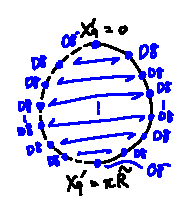
\includegraphics[width=11cm]{picture/type1dual}}
\caption{T-dual of Type I superstring theory.}
\label{type1dual}
\end{figure}
Note that an O$9^-$-plane splits into two O$8^-$-planes.
Accordingly, tension and RR-charge reduce by $2$.
In the end, T-dual of Type I on $S^1$ is
\begin{align}
 \textrm{Type I' } = \textrm{ Type IIA on } S^1/\ZZ_2 \quad \textrm{with} \quad  2 \textrm{ O$8^-$-plane }
 + (16+16) \textrm{ D$8$-branes }.
\end{align}

\subsection{\texorpdfstring{O$p$}{Op}-plane}

Of course, one can consider further T-dualities along other directions.  In particular, an
orientifold $p$-plane (O$p$) in Type II string theory is defined \cite{Dabholkar:1996pc,Dabholkar:1997zd} as the $\bZ_2$ involution
\be
\mathrm{O} p: \quad \mathbb{R}^{1, p} \times \mathbb{R}^{9-p} / {I}_{9-p} \Omega \cdot\begin{cases} 1 & p=0,1 \bmod 4 \\ (-1)^{F_{L}} & p=2,3 \bmod 4,\end{cases}
\ee
where ${I}_{9-p}$ is the involution of all coordinates in the transverse space $\mathbb{R}^{9-p}$ and $F_L$ is the left-moving spacetime fermion number operator. The presence of $(-1)^{F_{L}}$ for $p=2,3 \bmod 4$ can be understood from the requirement that the generator square to one on fermions. Due to the spacetime involution ${I}_{9-p}$ transverse to the O$p$-plane, the number of D$p$-branes parallel to the O$p$-plane is effectively doubled. Therefore, a stack of $n$ D$p$-branes along the O$p^-$-plane leads to an $\SO(2n)$ gauge theory (Dynkin type $D_{n}$) in Type II theory. To realize an $\SO(2n+1)$ gauge group (Dynkin type $B_{n+1}$), we need a combination of an O$p^-$-plane and $\frac12$ D$p$-brane, which is denoted by $\wt{\mathrm{O}p}^-$. Consequently, $n$ D$p$-branes with  $\wt{\mathrm{O}p}^-$-plane give rise to an $\SO(2n+1)$ gauge theory as a world-volume theory. As we will see in \S\ref{sec:Sdual}, it is natural to incorporate an $\wt{\mathrm{O}p}^+$-plane in Type II theory, which also gives rise to an $\Sp(k)$ gauge theory like an ${\mathrm{O}p}^+$-plane. They behave differently under the S-duality of Type IIB theory.


Each T-duality doubles the number of O-planes, and hence,
reduces the tension and the R-R charges.
Namely, we have the following relations:
\begin{align*}
 T_{\mathrm{O}p^\pm} = \pm 2^{p-5} \cdot T_{\mathrm{D}p} \quad (\textrm{tension}) \ , \quad
 \mu_{\mathrm{O}p^\pm} = \pm 2^{p-5} \cdot \mu_{\mathrm{D}p} \quad (\textrm{R-R charge}) \ .
\end{align*}
Since an $\wt{\mathrm{O}p}^-$-plane is  a combination of an O$p^-$-plane and $\frac12$ D$p$-brane, there is $\frac12$-shift in R-R charge as summarized in Table \ref{tab:Op}.
O$p$-planes bring richness to string theory such as quiver gauge theories,
the topology of $\RP^p$, real K-theory, Dirac quantization conditions, etc, which are beyond the scope of this lecture. We refer to \cite{Witten:1998xy,Hanany:2000fq,Hanany:1999sj,Tachikawa:2018njr} and references therein.

\begin{table}[ht]\centering
\begin{tabular}{|l|l|l|}
\hline O-plane & gauge group & RR-charge \\
\hline$\mathrm{O} p^{-}$ & $\SO(2 n)$ & $-2^{p-5}$ \\
 $\mathrm{O} p^{+}$ & $\Sp(2 n)$ & $+2^{p-5}$ \\
 $\widetilde{\mathrm{O}p}^{-}$ & $\SO(2 n+1)$ & $-2^{p-5}+\frac{1}{2}$ \\
 $\widetilde{\mathrm{O} p}^{+}$ & $\Sp(2 n)$ & $+2^{p-5}$ \\
\hline
\end{tabular}\label{tab:Op}
\end{table}

\end{document}
